\documentclass[border=6pt]{standalone}
\usepackage{tikz}
\usetikzlibrary{arrows.meta}
\begin{document}
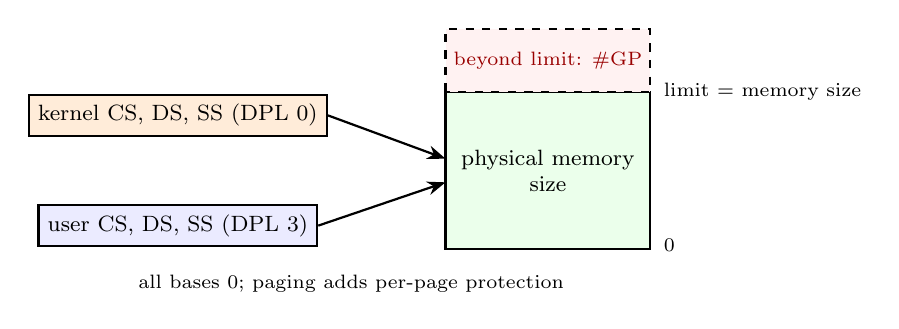
\begin{tikzpicture}[>=Stealth,font=\small]
\node[draw,thick,fill=orange!15,align=center,font=\footnotesize,minimum width=3.4cm] (k) at (0,0.7) {kernel CS, DS, SS (DPL 0)};
\node[draw,thick,fill=blue!8,align=center,font=\footnotesize,minimum width=3.4cm] (u) at (0,-0.7) {user CS, DS, SS (DPL 3)};
\draw[->,thick] (k.east) -- (3.4,0.15);
\draw[->,thick] (u.east) -- (3.4,-0.15);
\draw[thick,fill=green!8] (3.4,1.0) rectangle (6.0,-1.0);
\node[font=\footnotesize,align=center] at (4.7,0) {physical memory\\size};
\draw[thick,dashed,fill=red!5] (3.4,1.0) rectangle (6.0,1.8);
\node[font=\scriptsize,red!60!black] at (4.7,1.4) {beyond limit: \#GP};
\node[font=\scriptsize,anchor=west] at (6.05,-0.95) {0};
\node[font=\scriptsize,anchor=west,align=left] at (6.05,1.0) {limit = memory size};
\node[font=\scriptsize,anchor=north] at (2.2,-1.2) {all bases 0; paging adds per-page protection};
\end{tikzpicture}
\end{document}
